%%%%%%%%%%%%%%%%%%%%%%%%%%%%%%%%%%%%%%%%%
% Beamer Presentation
% LaTeX Template
% Note:
% data cleaning should be added
% https://realpython.com/python-data-cleaning-numpy-pandas/
% 


\documentclass{beamer}
\mode<presentation> {
\usetheme{Warsaw}
}

\usepackage{multicol}
\usepackage[russian]{babel}
\usepackage{graphicx} 
\usepackage{hyperref}

\title[Introduction to Python]{SQL with Python} 
\author{Sugarkhuu Radnaa} 
\institute[]
{
Py4Econ in Ulaanbaatar \\ 
\medskip
\textit{py4econ@gmail.com} 
}
\date{}  %15 January, 2022 \today

\begin{document}

\begin{frame}
\titlepage % Print the title page as the first slide
\end{frame}

\begin{frame}
    \frametitle{Week 4: Learning objectives}
    Get to know: 
    \begin{enumerate}
        \item Working with SQL using Python
    \end{enumerate}
\end{frame}

%------------------------------------------------
\section{Data types and structures} 
%------------------------------------------------

\begin{frame}
    \frametitle{SQL}
    SQL is the most popular database language. There are many different DBMS (database management system)s including SQL and NoSQL. \\
    \textbf{Popular SQL databases}:
    \begin{enumerate}
        \item Oracle SQL
        \item Microsoft SQL
        \item MySQL
        \item PostgreSQL
    \end{enumerate}    

    \textbf{Popular NoSQL databases}:
    \begin{enumerate}
        \item MongoDB
        \item ElasticSearch
        \item Casandra
    \end{enumerate}    
\end{frame}

\begin{frame}
    \centering
    \frametitle{Sample database (SQL) design}
    \begin{flushleft}
        Data architecture is a crucial in any organization. When due implemented, it can become a game changing factor. Efficient ETL, Datawarehouse and 
        data centers are necessary for an efficient DBMS.        
    \end{flushleft}
    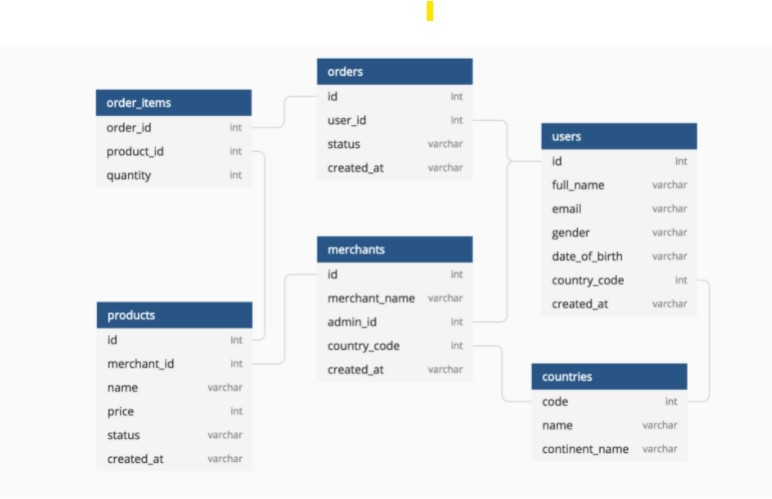
\includegraphics[scale=0.5]{figures/db_design.jpg}
\end{frame}

\begin{frame}
    \frametitle{SQL: W3SCHOOL examples}
    \begin{enumerate}
\tiny        \item SELECT CustomerName, City FROM Customers; 
        \item SELECT * FROM Customers
        WHERE Country='Mexico';
        \item SELECT * FROM Customers
        WHERE Country='Germany' AND (City='Berlin' OR City='München');
        \item UPDATE Customers
        SET ContactName = 'Alfred Schmidt', City= 'Frankfurt'
        WHERE CustomerID = 1;
        \item SELECT * FROM Customers
        WHERE ContactName LIKE 'a\%';
        \item SELECT Customers.CustomerName, Orders.OrderID
        FROM Customers
        LEFT JOIN Orders ON Customers.CustomerID = Orders.CustomerID
        ORDER BY Customers.CustomerName;
        \item SELECT COUNT(CustomerID), Country
        FROM Customers
        GROUP BY Country
        ORDER BY COUNT(CustomerID) DESC;
    \end{enumerate}
\end{frame}



%------------------------------------------------
\section{Homework} 
%------------------------------------------------

\begin{frame}
    \frametitle{Homework}
    \begin{enumerate}
        \item Task 1
    \end{enumerate}

    \vskip 2mm
    \begin{itemize}
        \item Push your result into your homework repository
        \item Deadline: 1 week %22 January, 2022
    \end{itemize}

\vfill
\textbf{Note:} Commit your results step by step.
\end{frame}

\begin{frame}
    \frametitle{Task 1}
    \begin{enumerate}
        \item Populate a MySQL (or PostgreSQL) table by the data in “data.xlsx” (CREATE TABLE)
        \item Select 'firstName' and 'lastName' of the first three rows  ('LIMIT')
        \item Select 'firstName' and 'age' of the last three rows ('ORDER BY, LIMIT')
    \end{enumerate}
\vfill
\textbf{Tip:} Watch the following tutorial for MySQL (PostgreSQL)
\begin{itemize}
    \item \href{https://www.youtube.com/watch?v=e1LPfehYSgg&list=PLS1QulWo1RIY4auvfxAHS9m_fZJ2wxSse}{MySQL}
    \item \href{https://www.youtube.com/watch?v=xaWlS9HtWYw}{PostgreSQL}
\end{itemize}
\end{frame}

\begin{frame}
\Huge{\centerline{Thank you!}}
\end{frame}

%----------------------------------------------------------------------------------------

\end{document} 